\section{Stationary variational inequality}
\subsection{}
\begin{frame}
\frametitle{Model problem and settings: contact between two membranes}
\vspace{-1.7 cm}
\begin{equation*}
\mbox{Find} \ u_1, u_2, \lambda \ \mbox{such that} \quad
\dps
\left\lbrace\begin{array}{llccc}
\dps -\mu_1 \Delta u_1-\lambda = f_1 \qquad \mbox{in} \quad \Omega, \\
\dps -\mu_2 \Delta u_2+\lambda = f_2 \qquad \mbox{in} \quad \Omega,\\
\textcolor{electricpurple}{u_1-u_2 \geq 0}, \quad 
\textcolor{carmine}{\lambda \geq 0}, \quad \dps (\textcolor{electricpurple}{u_1-u_2})\textcolor{carmine}{\lambda}=0 \quad \mbox{in} \quad \Omega, \hspace{0.2 cm}\\
\dps u_1=g > 0 \qquad \mbox{on} \quad\partial \Omega,\\
\dps u_2=0 \qquad \mbox{on} \quad\partial \Omega.
\end{array}
\right.
%\label{eq:modele_initial_membrane}
\end{equation*}
\vspace{-0.8 cm}
\begin{figure}
\begin{subfigure}[normal]{0.44\textwidth} 
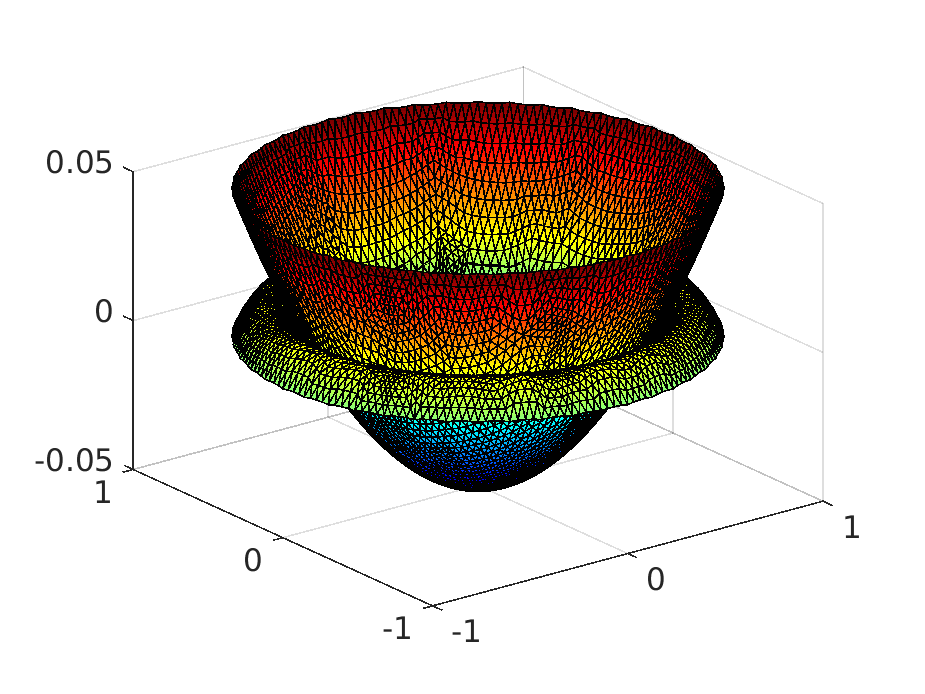
\includegraphics[width=\textwidth]{fig_article_chap_1/fig_membrane_cv.eps}    
\end{subfigure}
\qquad
\begin{subfigure}[normal]{0.44\textwidth}
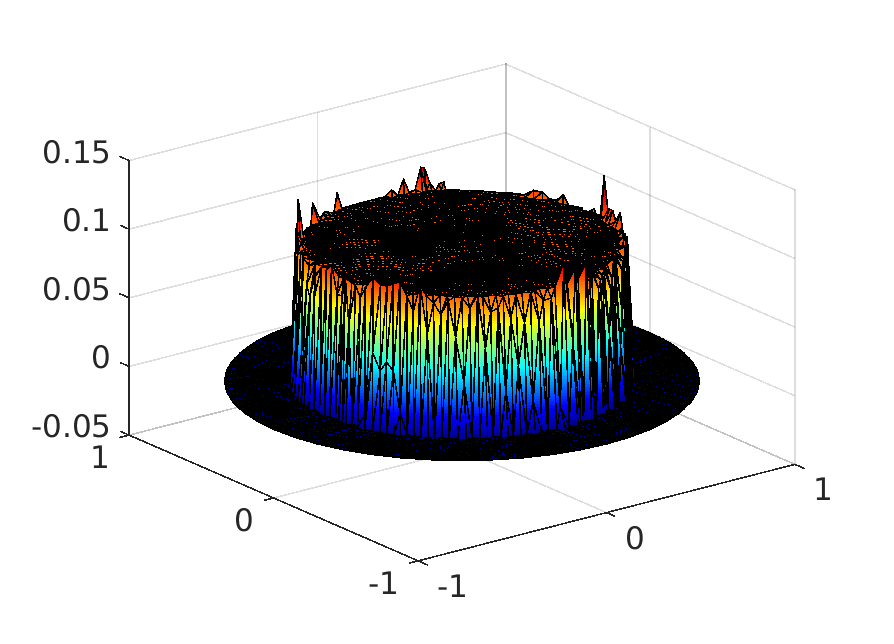
\includegraphics[width=\textwidth]{fig_article_chap_1/fig_lambda_cv.eps}     
\end{subfigure}
\end{figure}
\vspace*{-4.4cm}\hspace*{1.5 cm}$u_1$ \hspace{8 cm} $\lambda$\\
\vspace*{0.7cm}\hspace*{1.5 cm}$u_2$\\
\end{frame}
%
\begin{frame}
\frametitle{Continuous problem}
\begin{itemize}
\item $H_g^1(\Omega)\hspace{-0.1 cm} =\hspace{-0.1 cm} \left\{u\in H^1(\Omega), \hspace{0.1 cm} u=g \hspace{0.1 cm} \mbox{on} \hspace{0.1 cm} \partial \Omega\right\}$ \quad $\Lambda=\left\{\chi\in L^2(\Omega), \: \textcolor{carmine}{\chi \geq 0} \: \mbox{a.e.} \hspace{0.1 cm} \mbox{in} \ \Omega\right\}$
\end{itemize}
\textbf{Saddle point type weak formulation:}
For $(f_1,f_2)\in \left[L^2(\Omega)\right]^2$ and $g > 0$ find $(u_1,u_2,\lambda)\in H_g^1(\Omega)\times H_0^1(\Omega) \times \Lambda$ such that
\begin{equation*}
\begin{split}
& \dps \sum_{\ialf=1}^2 \mu_\ialf \left(\nab u_\ialf,\nab v_\ialf\right)_{\Omega} - \left(\lambda,v_1-v_2\right)_{\Omega} = \sum_{\ialf=1}^2\left(f_\ialf,v_\ialf\right)_{\Omega} \quad \forall (v_1,v_2) \in \left[H_0^1(\Omega)\right]^2 \\
& \left(\chi - \textcolor{carmine}{\lambda},\textcolor{electricpurple}{u_1-u_2}\right)_{\Omega} \geq 0 
\quad \forall \chi \in \Lambda 
\end{split}
 \tag{$\textcolor{electricpurple}{\mathrm{S}}$}
\end{equation*}
\hspace{4.5 cm}\textcolor{cadmiumgreen}{\textbf{equivalent to}}\\
\textbf{Variational inequality:}
\begin{itemize}
\item $\Kg= \left\{(v_1,v_2)\in H_g^1(\Omega)\times H_0^1(\Omega),\: \textcolor{electricpurple}{v_1-v_2 \geq 0} \; \; \mbox{a.e.} \ \mbox{in} 
\hspace{0.1 cm} \Omega \right\}$ \textcolor{midnightblue}{\textbf{convex}}
\end{itemize}
\begin{equation*}
\mbox{Find} \ \bu=\left(u_1,u_2\right) \in \Kg \ \mbox{s.t.} \ \dps \sum_{\ialf=1}^2 \mu_\ialf \left(\nab u_\ialf,\nab \left(v_\ialf-u_\ialf\right)\right)_{\Omega} \geq \sum_{\ialf=1}^2\left(f_\ialf,v_\ialf-u_\ialf\right)_{\Omega} \quad \forall \bv \in \Kg  \tag{$\textcolor{electricpurple}{\mathrm{R}}$}
\end{equation*}
\end{frame}
%
\begin{frame}
\textcolor{red}{\textbf{For any $p \geq 1$}}
\\
\frametitle{Discretization by finite elements}
\textcolor{cadmiumgreen}{\textbf{Spaces for the discretization:}}\\
$\Xghp=\left\{v_h \in \mathcal{C}^0(\overline{\Omega}),  {v_h}_{|K} \in \Pp (K), \ \forall K \in {\mathcal{T}}_h, \hspace{0.2 cm} v_h=g \hspace{0.2 cm} \mbox{on} \hspace{0.2 cm} \partial \Omega\right\}$\\
\vspace*{0.3 cm}
$\Xzerohp =\left\{v_h \in \calC^0(\overline{\Omega}); \ {v_h}|_{K} \in \Pp (K), \ \forall K \in \Th, \hspace{0.2 cm} v_h=0 \hspace{0.2 cm} \mbox{on} \hspace{0.2 cm} \partial \Omega \right\}$
\\
\vspace*{0.3 cm}
$\dps \Kghp=\left\{(\vunh,\vdeuxh) \in \Xghp \times \Xzerohp, \ \textcolor{electricpurple}{\vunh(\xl)-\vdeuxh(\xl)} \geq 0 \ \ \forall \xl \in \Vdp \right\} \textcolor{red}{\not \subset \Kg \quad \forall p \geq 2}$\\
\vspace*{0.2 cm}
\invisible<1>{
\textcolor{cadmiumgreen}{\textbf{Discrete variational inequality:}} find $\dps \uh=(\uunh,\udeuxh) \in \Kghp$ such that
\begin{equation*}
\dps \sum_{\ialf=1}^2 \mu_\ialf \left(\nab u_{\ialf h},\nab \left(v_{\ialf h}-u_{\ialf h}\right)\right)_{\Omega} \geq \sum_{\ialf=1}^2\left(f_\ialf,v_{\ialf h}-u_{\ialf h}\right)_{\Omega} \quad \forall \bv_h = (v_{1h},v_{2h})\in ~\Kghp \quad \textcolor{electricpurple}{(\mathrm{DR})}
\end{equation*}
\begin{center}
\textcolor{midnightblue}{Well-posed problem (Lions--Stampacchia)}
\end{center}
\invisible<2>{
\textcolor{midnightblue}{\textbf{Resolution techniques:}}
\footnotesize{Projected Newton methods (Bertsekas 1982), Active set Newton method (Kanzow 1999), Primal-dual active set strategy (Hinterm\"uller 2002).}
\invisible<3>{
}}}
\end{frame}
%
\begin{frame}
\frametitle{Saddle point formulation}
\only<1>{
Recall $\Lambda=\left\{\chi\in L^2(\Omega), \: \textcolor{carmine}{\chi \geq 0} \: \mbox{a.e.} \ \mbox{in} \hspace{0.1 cm} \Omega\right\}$
\\
\vspace{0.4 cm}
\textcolor{red}{\textbf{$p = 1$:}} \ $\Lahone \egaldef \left\{v_h \in \Xzerohone \  \textcolor{carmine}{v_h(\ba)} \geq 0 \ \forall \ba \in \mathcal{V}_{d}^{1,\mathrm{int}} \right\} \textcolor{red}{\bm \subset \bm \Lambda}$ \scriptsize{Ben Belgacem, Bernardi, Blouza, and Vohral{\'{\i}}k (2012)}.\\
\vspace{0.4 cm}
\normalsize{\textcolor{red}{\textbf{$p \geq 2$ (\textcolor{cadmiumgreen}{\textbf{new}}):}} \ $\Lahp \egaldef \left\{v_h \in \XXhp \ \left(v_h ,\psihl \right)_{\Omega} \geq 0 \ \forall \xl \in \Vdpint \ \left(v_h,\psihl\right)_{\Omega} = 0 \hspace{0.05 cm} \forall \xl \in \Vdpext\right\}$ $\textcolor{red}{\bm \not \subset \bm \Lambda}$}
\vspace{0.4 cm}
\begin{equation*}
\left\langle w_h ,v_h \right\rangle_h \egaldef \dps \sum_{\ba \in \Vh} w_h(\ba) v_h(\ba) \left(\psiha,1\right)_{\omah}  \quad \mbox{if} \quad \textcolor{red}{\textbf{$p=1$}} \quad \mbox{and} \quad \left \langle w_h ,v_h \right\rangle_h  \egaldef \dps \left(w_h, v_h\right)_{\Omega} \quad \mbox{if} \quad \textcolor{red}{\textbf{$p \geq 2$}}
\end{equation*}
% \vspace{0.2 cm}
% \textcolor{cadmiumgreen}{\textbf{Continuous weak formulation}}
% \begin{equation*}
% \begin{split}
% & \dps \sum_{\ialf=1}^2 \mu_\ialf \left(\nab u_\ialf,\nab v_\ialf\right)_{\Omega} - \left(\lambda,v_1-v_2\right)_{\Omega} = \sum_{\ialf=1}^2\left(f_\ialf,v_\ialf\right)_{\Omega} \quad \forall (v_1,v_2) \in \left[H_0^1(\Omega)\right]^2 \\
% & \left(\chi - \textcolor{carmine}{\lambda},\textcolor{electricpurple}{u_1-u_2}\right)_{\Omega} \geq 0 
% \quad \forall \chi \in \Lambda 
% \end{split}
%  \tag{$\textcolor{electricpurple}{\mathrm{S}}$}
% \end{equation*}
}
\only<2>{
Recall $\Lambda=\left\{\chi\in L^2(\Omega), \: \textcolor{carmine}{\chi \geq 0} \: \mbox{a.e.} \ \mbox{in} \hspace{0.1 cm} \Omega\right\}$
\\
\vspace{0.4 cm}
\textcolor{red}{\textbf{$p = 1$:}} \ $\Lahone \egaldef \left\{v_h \in \Xzerohone \  \textcolor{carmine}{v_h(\ba)} \geq 0 \ \forall \ba \in \mathcal{V}_{d}^{1,\mathrm{int}} \right\} \textcolor{red}{\bm \subset \bm \Lambda}$ \scriptsize{Ben Belgacem, Bernardi, Blouza, and Vohral{\'{\i}}k (2012)}.\\
\vspace{0.4 cm}
\normalsize{\textcolor{red}{\textbf{$p \geq 2$ (\textcolor{cadmiumgreen}{\textbf{new}}):}} \ $\Lahp \egaldef \left\{v_h \in \XXhp \ \left(v_h ,\psihl \right)_{\Omega} \geq 0 \ \forall \xl \in \Vdpint \ \left(v_h,\psihl\right)_{\Omega} = 0 \hspace{0.05 cm} \forall \xl \in \Vdpext\right\}$ $\textcolor{red}{\bm \not \subset \bm \Lambda}$} 
\vspace{0.4 cm}
\begin{equation*}
\left\langle w_h ,v_h \right\rangle_h \egaldef \dps \sum_{\ba \in \Vh} w_h(\ba) v_h(\ba) \left(\psiha,1\right)_{\omah}  \quad \mbox{if} \quad \textcolor{red}{\textbf{$p=1$}} \quad \mbox{and} \quad \left \langle w_h ,v_h \right\rangle_h  \egaldef \dps \left(w_h, v_h\right)_{\Omega} \quad \mbox{if} \quad \textcolor{red}{\textbf{$p \geq 2$}}
\end{equation*}
\vspace{0.2 cm}
\textcolor{cadmiumgreen}{\textbf{Continuous weak formulation}}
\begin{equation*}
\begin{split}
& \dps \sum_{\ialf=1}^2 \mu_\ialf \left(\nab u_\ialf,\nab v_\ialf\right)_{\Omega} - \left(\lambda,v_1-v_2\right)_{\Omega} = \sum_{\ialf=1}^2\left(f_\ialf,v_\ialf\right)_{\Omega} \quad \forall (v_1,v_2) \in \left[H_0^1(\Omega)\right]^2 \\
& \left(\chi - \textcolor{carmine}{\lambda},\textcolor{electricpurple}{u_1-u_2}\right)_{\Omega} \geq 0 
\quad \forall \chi \in \Lambda 
\end{split}
 \tag{$\textcolor{electricpurple}{\mathrm{S}}$}
\end{equation*}
}

\only<3>{
Recall $\Lambda=\left\{\chi\in L^2(\Omega), \: \textcolor{carmine}{\chi \geq 0} \: \mbox{a.e.} \ \mbox{in} \hspace{0.1 cm} \Omega\right\}$
\\
\vspace{0.4 cm}
\textcolor{red}{\textbf{$p = 1$:}} \ $\Lahone \egaldef \left\{v_h \in \Xzerohone \  \textcolor{carmine}{v_h(\ba)} \geq 0 \ \forall \ba \in \mathcal{V}_{d}^{1,\mathrm{int}} \right\} \textcolor{red}{\bm \subset \bm \Lambda}$ \scriptsize{Ben Belgacem, Bernardi, Blouza, and Vohral{\'{\i}}k (2012)}.\\
\vspace{0.4 cm}
\normalsize{\textcolor{red}{\textbf{$p \geq 2$ (\textcolor{cadmiumgreen}{\textbf{new}}):}} \ $\Lahp \egaldef \left\{v_h \in \XXhp \ \left(v_h ,\psihl \right)_{\Omega} \geq 0 \ \forall \xl \in \Vdpint \ \left(v_h,\psihl\right)_{\Omega} = 0 \hspace{0.05 cm} \forall \xl \in \Vdpext\right\}$ $\textcolor{red}{\bm \not \subset \bm \Lambda}$} 
\vspace{0.4 cm}
\begin{equation*}
\left\langle w_h ,v_h \right\rangle_h \egaldef \dps \sum_{\ba \in \Vh} w_h(\ba) v_h(\ba) \left(\psiha,1\right)_{\omah}  \quad \mbox{if} \quad \textcolor{red}{\textbf{$p=1$}} \quad \mbox{and} \quad \left \langle w_h ,v_h \right\rangle_h  \egaldef \dps \left(w_h, v_h\right)_{\Omega} \quad \mbox{if} \quad \textcolor{red}{\textbf{$p \geq 2$}}
\end{equation*}
\vspace{0.2 cm}
\textcolor{cadmiumgreen}{\textbf{Discrete weak formulation}}
Find $(\uunh,\udeuxh,\lambh)\in \Xghp \times \Xzerohp \times
\Lahp$ s.t. $\forall(z_{1h},z_{2h})\in [\Xzerohp]^2$ 
\vspace{-0.3 cm}
\begin{equation*}
\begin{split}
& \sum_{\ialf=1}^2 \mu_\ialf \left(\nab u_{\ialf h}, \nab z_{\ialf h}\right)_{\Omega}
- \left\langle \lambh, z_{1h}-z_{2h} \right \rangle_h
= \sum_{\ialf=1}^2 \left(f_\ialf,z_{\ialf h}\right)_{\Omega}, \\
& \left\langle \chi_h - \textcolor{carmine}{\lambh}, \textcolor{electricpurple}{\uunh - \udeuxh}\right \rangle_h   \geq 0 \quad \forall \chi_h \in \Lahp.
\end{split}
 \tag{$\textcolor{electricpurple}{\mathrm{DS}}$}
\end{equation*}
}
\end{frame} 
%

\begin{frame}
\frametitle{Discrete complementarity problems}
\vspace{-1 cm}
\begin{equation*}
\begin{array}{lcl}
\dps \sum_{\ialf=1}^2 \mu_\ialf \left(\nab u_{\ialf h}, \nab z_{\ialf h}\right)_{\Omega}
- \left\langle \lambh, z_{1h}-z_{2h} \right \rangle_h
=  \dps \sum_{\ialf=1}^2 \left(f_\ialf,z_{\ialf h}\right)_{\Omega} \quad \forall(z_{1h},z_{2h})\in [\Xzerohp]^2, \\
\textcolor{electricpurple}{\left(\uunh-\udeuxh \right)(\xl)} \geq 0 \ \forall \xl \in \Vdpint, \ \left\langle \textcolor{carmine}{\lambh}, \psihl \right \rangle_h \geq 0 \ \forall \xl \in \Vdpint, \ \left\langle \textcolor{carmine}{\lambh}, \textcolor{electricpurple}{\uunh - \udeuxh} \right \rangle_h=0.  \quad \textcolor{electricpurple}{(\mathrm{DS}2)}
\end{array}
\end{equation*}
\invisible<1>{
\textcolor{cadmiumgreen}{\textbf{Matrix representation of \textcolor{electricpurple}{($\mathrm{DS}2)$}}}
\newline
\newline
\invisible<2>{
\textcolor{red}{\textbf{$p \geq 1$:}}
$\dps \uunh = \sum_{l=1}^{\Ndpint} \left(\X_{1h} \right)_l \psihl + g, \quad \udeuxh = \sum_{l=1}^{\Ndpint} \left(\X_{2h} \right)_l \psihl \quad \lambh = \sum_{l=1}^{\Ndpint} \left(\X_{3h} \right)_l \Thetahl.$ 
\begin{equation*}
\begin{split}
&\bbE \Xh = \bF,\\
&\textcolor{electricpurple}{\X_{1h} + g {\bf 1} - \X_{2h}} \geq 0, \quad \textcolor{carmine}{\X_{3h}} \geq 0, \quad \left(\textcolor{electricpurple}{\X_{1h} + g {\bf 1} - \X_{2h}} \right) \cdot \textcolor{carmine}{\X_{3h}} = 0.
\end{split}
\quad 
\bbE
\egaldef
\left[\begin{array}{ccr}
\mu_1 \bbS & \mathbf{0} & -\mathbb{D} \\
\mathbf{0} &\mu_2 \bbS & + \mathbb{D}
\end{array}
\right]
\end{equation*}
\invisible<3>{
}}}
%% EXPRESSION OF THE CONSTRAINTS IN THE LAGRANGE BASIS FOR P SUP 2
% \begin{onlyenv}<2>
%  \textcolor{red}{\textbf{$p \geq 2$: Lagrange basis:}}
% The discrete lagrange multiplier $\lambh$ is decomposed in the full space $\XXhp$ as 
% \beeqn
% \lambh = \sum_{l=1}^{\Ndp} \left(\widetilde{\X}_{3h}\right)_l \psihl \quad \mbox{with} \quad \widetilde{\X}_{3h} \in \R^{\Ndp}.
% \eeqn
% \beeqn
% \begin{split}
% &\widetilde{\bbE}_p \Xh = \bF,\\
% &\textcolor{electricpurple}{\X_{1h} + g {\bf 1} - \X_{2h}} \geq 0
% , \quad \textcolor{carmine}{\widehat{\mathbb{M}} \widetilde{\X}_{3h}} \geq 0, \quad 
% \left(\textcolor{electricpurple}{\X_{1h} + g {\bf 1} - \X_{2h}} \right) \cdot \textcolor{carmine}{\widehat{\mathbb{M}} \widetilde{\X}_{3h}} = 0.
% \end{split}
% \widetilde{\bbE}_p
% \egaldef
% \left[\begin{array}{ccr}
% \mu_1 \bbS & \mathbf{0} & -\widehat{\mathbb{M}} \\
% \mathbf{0} &\mu_2 \bbS & + \widehat{\mathbb{M}}
% \end{array}
% \right]
% \eeqn
% \end{onlyenv}

%% BASE DUALE
% \textcolor{red}{\textbf{$p \geq 2$: Dual basis:}}
% The discrete Lagrange multiplier $\lambh$ is decomposed in the basis $\Thetahl$ as
% \beeqn
% \lambh = \sum_{l=1}^{\Ndpint} \left(\X_{3h} \right)_l \Thetahl, \quad \mbox{with} \quad \X_{3h} \in \R^{\Ndpint}.
% \eeqn
% \beeqn
% \begin{split}
% & \bbE_{p} \Xh = \bF,\\
% & \textcolor{electricpurple}{\X_{1h} + g {\bf 1} - \X_{2h}} \geq 0, \quad \textcolor{carmine}{\X_{3h}} \geq 0, \quad \left(\textcolor{electricpurple}{\X_{1h} + g {\bf 1} - \X_{2h}}\right) \cdot \textcolor{carmine}{\X_{3h}}=0. 
% \end{split}
% \qquad 
% \bbE_{p}
% \egaldef
% \left[\begin{array}{ccr}
% \mu_1 \bbS & \mathbf{0} & - \mathbb{I}_{\mathrm{d}}\\
% \mathbf{0} &\mu_2 \bbS & + \mathbb{I}_{\mathrm{d}}
% \end{array}
% \right]
% \eeqn
% \end{onlyenv}
\end{frame}
%
\begin{frame}[noframenumbering]
 \begin{center}
 \Huge{\textcolor{carmine}{Resolution}}
\end{center}

\end{frame}
%\begin{frame}
%\begin{onlyenv}<1>
%slide1
% \end{onlyenv}
% \begin{onlyenv}<2>
% slide2
% \end{onlyenv}
% \begin{onlyenv}<3>
% slide3
% \end{onlyenv}
% \begin{onlyenv}<4>
% slide4
% \end{onlyenv}
% \end{frame}
%
%
\begin{frame}
\frametitle{C-functions}
\vspace{-0.2 cm}
\begin{definition}
$f: \left(\R^m\right)^2  \rightarrow \R^m$ ($m \geq 1$) is a
$C$-function or a complementarity function if
\begin{equation*}
\forall(\bx,\by)\in \left(\R^m\right)^2
\qquad f(\bx,\by)=\mathbf{0} \quad \iff \quad
\bx \geq \mathbf{0}, \quad \by \geq \mathbf{0}, \quad \bx {\cdot} \by=0.
\end{equation*}
\end{definition}
\invisible<1>{
\textcolor{cadmiumgreen}{\textbf{min function:}} \ $\left(\min \{\bx, \by\}\right)_l \egaldef \min \left\{\bx_l, \by_l\right\} \qquad l = 1,\dots, m$\\
\vspace{0.2 cm}
\invisible<2>{ \textcolor{cadmiumgreen}{\textbf{ Fischer--Burmeister function:}} \ $\left(f_{\mathrm{FB}}(\bx,\by)\right)_l \egaldef \sqrt{\bx_l^2+\by_l^2}-\left(\bx_l+\by_l\right) \quad  l = 1,\dots, m$% \\
% & \mbox{\textcolor{cadmiumgreen}{\textbf{Mangasarian function:}}} \ \left(f_{\mathrm{M}}(\bx,\by)\right)_l \egaldef \xi (|\bx_l-\by_l|) - \xi(\by_l) - \xi(\bx_l)  \quad  l = 1,\dots, m, 
% where $\xi: \R \mapsto \R$ is an increasing function satisfying $\xi(\bm 0)=\bm 0$.
\\ 
\invisible<3>{$\bx=\textcolor{electricpurple}{\X_{1h} + g {\bf 1} - \X_{2h}}$, \ $\by = \textcolor{carmine}{\X_{3h}}$ ($m=\Ndpint$), \ $\CFun(\X_{h})
= \tilde \CFun(\textcolor{electricpurple}{\X_{1h} + g {\bf 1} - \X_{2h},} \textcolor{carmine}{\X_{3h}})$. 
\begin{equation*}
\left\lbrace\begin{array}{llccc}
\bbE \X_{h} &= \bF,\\
\CFun(\X_{h})&=\mathbf{0}.
\end{array}
\right.
\end{equation*}
\invisible<4>{
\textcolor{red}{\textbf{The C-function is not Fréchet differentiable.}}\\
\vspace{0.2 cm}
\invisible<5>{
\textcolor{red}{\textbf{We will use semismooth Newton algorithms.}} 
\\
\scriptsize{Facchinei and Pang (2003), Bonnans, Gilbert, Lemar\'echal, and Sagastiz\'abal (2006).} 
\invisible<6>{
}}}}}}
\end{frame}
%
\begin{frame}
\frametitle{Inexact semismooth Newton method}
\begin{onlyenv}<1>
\textcolor{cadmiumgreen}{\textbf{Newton initial vector:}} $\Xh^{\zzero} \egaldef \left(\X_{1h}^{\zzero},\X_{2h}^{\zzero}, \X_{3h}^{\zzero} \right)^{T} \in \R^{3 \Ndpint}$, on step $\kk \geq 1$, one looks for $\Xh^{\kk} \in \R^{3 \Ndpint}$ such that
\begin{equation*}
\bbA^{\kk-1}\Xh^{\kk}=\bB^{\kk-1},
\end{equation*} 
where 
%the square matrix $\bbA^{\kk-1}$ and the right-hand side vector $\bB^{\kk-1}$ are respectively defined by
\begin{equation*}
\dps \bbA^{\kk-1}\egaldef
\left[\begin{array}{c}
\bbE \\
\JacCFun(\Xh^{\kk-1})
\end{array}
\right],
\quad  \hspace{0.1 cm} \bB^{\kk-1} \egaldef
\left[\begin{array}{c}
\bF\\
\JacCFun(\Xh^{\kk-1})\Xh^{\kk-1}-\CFun(\Xh^{\kk-1})
\end{array}
\right].
%\quad  \forall k\geq 1.
\end{equation*}
\end{onlyenv}
\begin{onlyenv}<2>
\textcolor{cadmiumgreen}{\textbf{Newton initial vector:}} $\Xh^{\zzero} \egaldef \left(\X_{1h}^{\zzero},\X_{2h}^{\zzero}, \X_{3h}^{\zzero} \right)^{T} \in \R^{3 \Ndpint}$, on step $\kk \geq 1$, one looks for $\Xh^{\kk} \in \R^{3 \Ndpint}$ such that
\begin{equation*}
\bbA^{\kk-1}\Xh^{\kk}=\bB^{\kk-1},
\end{equation*} 
where 
%the square matrix $\bbA^{\kk-1}$ and the right-hand side vector $\bB^{\kk-1}$ are respectively defined by
\begin{equation*}
\dps \bbA^{\kk-1}\egaldef
\left[\begin{array}{c}
\bbE \\
\JacCFun(\Xh^{\kk-1})
\end{array}
\right],
\quad  \hspace{0.1 cm} \bB^{\kk-1} \egaldef
\left[\begin{array}{c}
\bF\\
\JacCFun(\Xh^{\kk-1})\Xh^{\kk-1}-\CFun(\Xh^{\kk-1})
\end{array}
\right].
%\quad  \forall k\geq 1.
\end{equation*}
\textcolor{cadmiumgreen}{\textbf{Inexact solver initial vector:}}
$\Xh^{\kk,\izzero} \in \R^{3 \Ndpint}$, often taken as $\Xh^{\kk,\izzero} = \Xh^{\kk-1}$, this yields on step $\ii \geq
1$ an approximation $\Xh^{\kk,\ii}$ to $\Xh^{\kk}$ satisfying
\begin{equation*}
\bbA^{\kk-1}\Xh^{\kk,\ii} =\bB^{\kk-1}-{\bm R}_h^{\kk,\ii},
\end{equation*}
where ${\bm R}_h^{\kk,\ii} \in \R^{3 \Ndpint}$ is the algebraic residual vector.
\end{onlyenv}

\begin{onlyenv}<3>
\begin{center}
\Huge{\textcolor{carmine}{A posteriori error estimates}}
\end{center}
\end{onlyenv}
\end{frame}
%
\begin{frame}
\frametitle{A posteriori analysis}
\begin{equation*}
\tnorm{\bu-\bu_h^{\kk,\ii}}_{\Omega} \egaldef \left(\sum_{\ialf = 1}^2 \mu_\ialf \left\|\nab \left(\uialf-\uialfh^{\kk,\ii} \right)\right\|_{\Omega}^2 \right)^{\frac{1}{2}} \leq \eta^{\kk,\ii} \egaldef \left(\sum_{K \in Th}\left[\eta_{K}(\bu_h^{\kk,\ii}) \right]^2\right)^{\frac{1}{2}}
\end{equation*}
\begin{itemize}
\item $\eta_{K}(\bu_h^{\kk,\ii})$ local estimator depending on the approximate solution 
\item $\eta^{\kk,\ii} \leq \eta_{\mathrm{disc}}^{\kk,\ii} + \eta_{\mathrm{lin}}^{\kk,\ii} + \eta_{\mathrm{alg}}^{\kk,\ii}$: identification of the error components
\item $\eta_{K}(\bu_h^{\kk,\ii}) \leq$ local error + $\underbrace{\mathrm{local \ contact \ term}}_{\mathrm{\textcolor{midnightblue}{typically \ very \ small}}}$: local efficiency
\item adaptive inexact stopping criteria based on the error components
\end{itemize} 
\invisible<1>{
\textcolor{red}{We employ the methodology of equilibrated flux reconstruction to obtain local error estimators.}
\newline 
\footnotesize{Destuynder \& M\'etivet (1999) Braess \& Sch\"oberl (2008), Ern \& Vohral{\'{\i}}k (2013)}
\invisible<2>{
}}
\end{frame}
%
\begin{frame}
\frametitle{Component flux reconstruction}
\textcolor{cadmiumgreen}{\textbf{Motivation:}}
\begin{equation*}
-\mu_\ialf \nab u_{\ialf} \in \HdivOmeg,  \quad  -\mu_\ialf \nab u_{\ialf h}^{\kk,\ii} \not \in \HdivOmeg, \quad \nab {\cdot} \left(-\mu_\ialf \nab u_{\ialf h}^{\kk,\ii} \right) \neq f_\ialf -(-1)^{\ialf} \lambh^{\kk,\ii}
\end{equation*}
\invisible<1>{
\textcolor{cadmiumgreen}{\textbf{Flux reconstruction:}}
\begin{equation*}
{\bm \sigma}_{\ialf h}^{\kk,\ii} \in \HdivOmeg \quad \left(\nab {\cdot} {\bm \sigma}_{\ialf h}^{\kk,\ii}, 1 \right)_K = \left( f_\ialf -(-1)^{\ialf} \lambh^{\kk,\ii}, 1  \right)_K 
\end{equation*}
\invisible<2>{
\textcolor{cadmiumgreen}{\textbf{Decomposition of the flux:}}
\begin{equation*}
{\bm \sigma}_{\ialf h}^{\kk,\ii}  = {\bm \sigma}_{\ialf h, \mathrm{alg}}^{\kk,\ii} + {\bm \sigma}_{\ialf h, \mathrm{disc}}^{\kk,\ii}
\end{equation*}
\invisible<3>{
\textcolor{cadmiumgreen}{\textbf{Algebraic error flux reconstruction:}}
\begin{equation*}
{\bm \sigma}_{\ialf h, \mathrm{alg}}^{\kk,\ii} \in \HdivOmeg \quad \nab {\cdot} {\bm \sigma}_{\ialf h, \mathrm{alg}}^{\kk,\ii}=r_{\ialf h}^{\kk,\ii} \quad \mbox{where} \quad r_{\ialf h}^{\kk,\ii} \quad \mbox{is the functional representation of} \quad {\bm R}_{\ialf h}^{\kk,\ii}
\end{equation*}
\scriptsize{Pape{\v z}, R{\"u}de, Vohral{\'{\i}}k and Wohlmuth (2017).}
\newline
\invisible<4>{
\normalsize{\textcolor{cadmiumgreen}{\textbf{Discretization flux reconstruction:}}
\begin{equation*}
{\bm \sigma}_{\ialf h, \mathrm{disc}}^{\kk,\ii} \in \HdivOmeg \quad \left(\nab {\cdot} {\bm \sigma}_{\ialf h,\mathrm{disc}}^{\kk,\ii}, 1 \right)_K = \left( f_\ialf -(-1)^{\ialf} \lambh^{\kk,\ii} - r_{\ialf h}^{\kk,\ii}, 1  \right)_K
\end{equation*}
}
\invisible<5>{
}}}}}
\end{frame}
%
%%%%ALG FLUX RECONSTRUCTION
% \begin{frame}
% \frametitle{Algebraic flux reconstruction}
% \vspace*{-0.5 cm}
% \begin{equation*}
% \begin{array}{lclcc}
% \left({\bm \sigma}_{\ialf j,\mathrm{alg}}^{\kk,\ii,\ba}, \tauj\right)_{\omajminusun}-\left(\gamma_{\ialf j}^{\kk,\ii,\ba},\nab {\cdot} \tauj\right)_{\omajminusun} &=& 0 & \forall \tauj\in \Vspacejjmuna, \\
% \left(\nab {\cdot} {\bm \sigma}_{\ialf j,\mathrm{alg}}^{\kk,\ii,\ba}, q_{j}\right)_{\omajminusun}&=&\dps\left(\tilde{g}_{\ialf j}^{\kk,\ii,\ba}, q_{j}\right)_{\omajminusun} & \forall q_{j} \in \Qspacejjmuna,
% \end{array}
% \end{equation*}
% \vspace{-0.8 cm}
% \begin{minipage}[c]{.55 \linewidth}
% \vspace{-0.8 cm}
% \begin{equation*}
% \begin{split}
% \Vspacejjmuna &\egaldef \left\{ \tauj \in \RTp(\omajminusun),
% \ \tauj {\cdot} \nnomajminusun =0 \mbox{ on } \partial \omajminusun \right\}, \\
% \Qspacejjmuna &\egaldef \Pp^{0}({\omajminusun}), \ \ba \in \mathcal{V}_{j-1}^{\mathrm{int}}
% \end{split}
% \end{equation*}
% \vspace{-0.2 cm}
% \invisible<1-2>{
% \begin{equation*}
% \begin{split}
% \Vspacejjmuna & \egaldef\left\{ \tauj \in \RTp(\omajminusun),
% \ \tauj {\cdot} \nnomajminusun=0 \  \mbox{on} \ \partial \omajminusun \backslash \partial \Omega\right\},
% \\
% \Qspacejjmuna & \egaldef \Pp({\omajminusun}), \ \ba \in \mathcal{V}_{j-1}^{\mathrm{ext}}
% \end{split}
% \end{equation*}
% }
% \end{minipage}
% \hfill
% \begin{minipage}[c]{.42 \linewidth}
% \hspace{3 cm}
% \begin{figure}
%   \begin{overprint}
%     \onslide<1>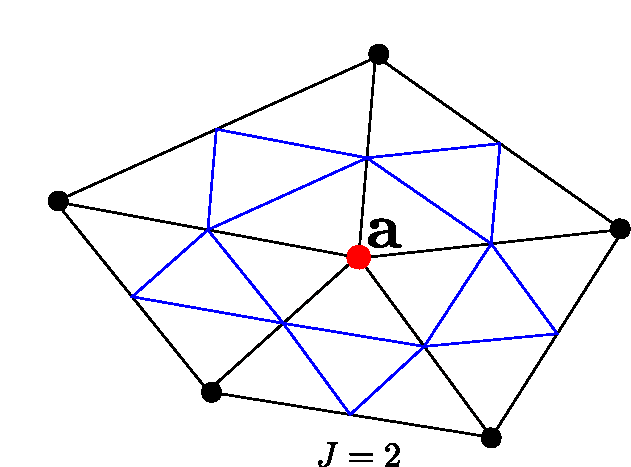
\includegraphics[width=0.9 \textwidth]{patch_alg_1.pdf}
%     \onslide<2>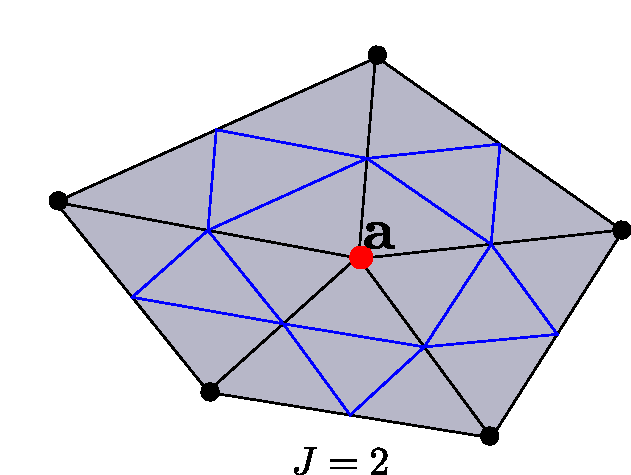
\includegraphics[width=0.9 \textwidth]{patch_alg_2.pdf}
%     \onslide<3>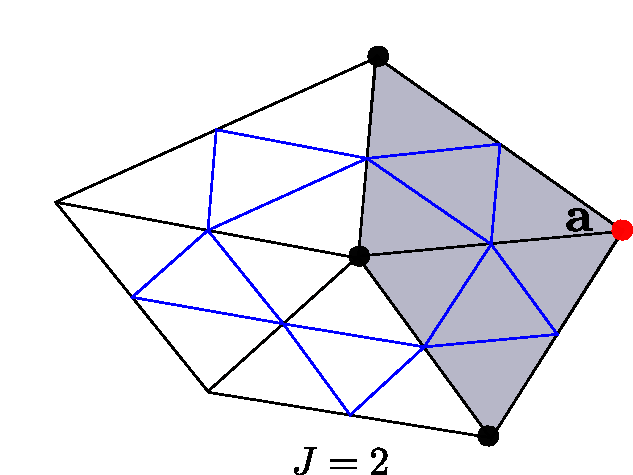
\includegraphics[width=0.9 \textwidth]{patch_alg_2_bis.pdf}
%     \onslide<4>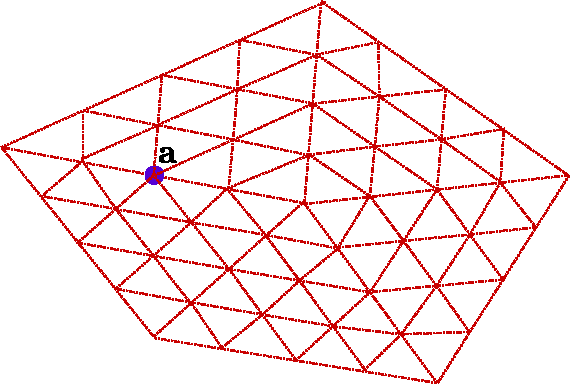
\includegraphics[width=0.9 \textwidth]{patch_alg_3.pdf}
%     \onslide<5->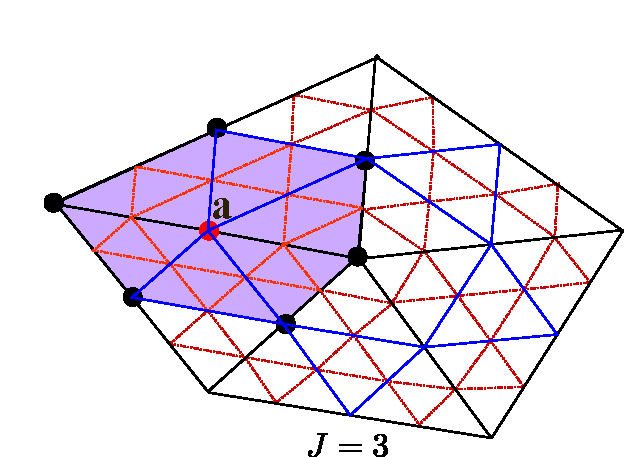
\includegraphics[width=0.9 \textwidth]{patch_alg_4.pdf} 
%     \end{overprint}
% \end{figure}
% \end{minipage}
% \vspace{-0.2 cm}
% \invisible<1-4>{
% \begin{equation*}
% {\bm \sigma}_{\ialf j,\mathrm{alg}}^{\kk,\ii} \egaldef \sum_{j=1}^{J} \sum_{\ba \in \mathcal{V}_{j-1}} {\bm \sigma}_{\ialf j,\mathrm{alg}}^{\kk,\ii,\ba}
% \end{equation*}
% }
% \end{frame}
%
%
\begin{frame}
\frametitle{Estimators}

\textcolor{cadmiumgreen}{\textbf{Violations of physical properties of the numerical solution}}
\begin{equation*}
{\bm \sigma}_{\ialf h}^{\kk,\ii} \neq -\nab \uialfh^{\kk,\ii}, \qquad \nab {\cdot} {\bm \sigma}_{\ialf h}^{\kk,\ii} \neq f_\ialf -(-1)^{\ialf} \lambh^{\kk,\ii}
\end{equation*}
\invisible<1>{
\textcolor{midnightblue}{\textbf{Flux estimator:}}
\begin{equation*}
\eta_{\mathrm{F},K,\ialf}^{\kk,\ii} \egaldef \left\|\mu_\ialf^{\frac{1}{2}} \nab u_{\ialf h}^{\kk,\ii}
+\mu_\ialf^{-\frac{1}{2}} {\bm \sigma}_{\ialf h}^{\kk,\ii}\right\|_{K},
\end{equation*}
\textcolor{midnightblue}{\textbf{Residual estimator:}}
\begin{equation*}
\eta_{\mathrm{R},K,\ialf}^{\kk,\ii} \egaldef \frac{h_K}{\pi} \mu_\ialf^{-\frac{1}{2}}
\left\|f_\ialf - \nab {\cdot} {\bm \sigma}_{\ialf h}^{\kk,\ii} -(-1)^{\ialf} \lambh^{\kk,\ii} \right\|_{K},
\end{equation*}
\invisible<2>{
}}
\end{frame}
%
\begin{frame}
\textcolor{cadmiumgreen}{ \textbf{Violations of the complementarity constraints}}\\
\invisible<1>{
\textcolor{red}{p = 1:} \ \textcolor{midnightblue}{\textbf{at convergence:}} 
\vspace{-0.1 cm}
\begin{equation*} 
(\uunh \hspace{-0.05 cm} - \hspace{-0.05 cm} \udeuxh)(\ba) \hspace{-0.05 cm} \geq \hspace{-0.05 cm} 0 \hspace{-0.05 cm} \Rightarrow \hspace{-0.05 cm} \uh \hspace{-0.05 cm} \in \hspace{-0.05 cm} \Kg, \hspace{0.1 cm} \lambh(\ba) \hspace{-0.05 cm} \geq \hspace{-0.05 cm} 0 \hspace{-0.05 cm} \Rightarrow \hspace{-0.05 cm} \lambh \hspace{-0.05 cm} \in \hspace{-0.05 cm} \Lambda, \hspace{0.1 cm} \lambh(\ba) \hspace{-0.05 cm} \cdot \hspace{-0.05 cm} (\uunh \hspace{-0.05 cm} - \hspace{-0.05 cm} \udeuxh)(\ba) \hspace{-0.05 cm} = \hspace{-0.05 cm} 0 \textcolor{red}{\bm{\not \Rightarrow}} \lambh \hspace{-0.05 cm} \cdot \hspace{-0.05 cm} (\uunh \hspace{-0.05 cm} - \hspace{-0.05 cm} \udeuxh) \hspace{-0.05 cm} = \hspace{-0.05 cm} 0
\end{equation*}
\invisible<2>{
\textcolor{red}{p = 1:} \ \textcolor{midnightblue}{\textbf{at each inexact semismooth step:}}
\begin{equation*}
(\uunh^{\kk,\ii}-\udeuxh^{\kk,\ii})(\ba) \not \geq 0 \quad \lambh^{\kk,\ii}(\ba) \not \geq 0 \quad \lambh^{\kk,\ii}(\ba) \cdot (\uunh^{\kk,\ii}-\udeuxh^{\kk,\ii})(\ba)\not=0 \quad \forall \ba \in \Vhint
\end{equation*}
\invisible<3>{
\textcolor{red}{$p \geq 2$:} \ \textcolor{midnightblue}{\textbf{at convergence:}} 
\vspace{-0.1 cm}
\begin{equation*}
(\uunh - \udeuxh)(\bx_l) \geq 0 \ \textcolor{red}{\bm{\not \Rightarrow}} \ \uh \in \Kg \ , \ \left(\lambh,\psihl \right)_{\Omega} \geq 0 \ \textcolor{red}{\bm{\not \Rightarrow}} \ \lambh \in \Lambda  
\end{equation*}
\begin{equation*}
\left(\lambh,\uunh-\udeuxh\right)_{\Omega} = 0 \ \textcolor{red}{\bm{\not \Rightarrow}} \ \lambh \cdot \left(\uunh-\udeuxh\right) = 0
\end{equation*}
\invisible<4>{
\textcolor{red}{$p \geq 2$:} \ \textcolor{midnightblue}{\textbf{at each inexact semismooth step:}}
\begin{equation*}
(\uunh^{\kk,\ii} - \udeuxh^{\kk,\ii})(\bx_l) \not \geq 0 \ , \ \left(\lambh^{\kk,\ii},\psihl \right)_{\Omega} \not \geq 0 \ \forall \bx_l \in \Vdpint \ \left(\lambh^{\kk,\ii},\uunh^{\kk,\ii}-\udeuxh^{\kk,\ii}\right)_{\Omega} \neq 0
\end{equation*}
\invisible<5>{
\textcolor{midnightblue}{\textbf{Contact estimator:}}
\begin{equation*}
\eta_{\mathrm{C},K}^{\kk,\ii} \egaldef 2 \left(\lambh^{\kk,\ii,\mathrm{pos}},\uunh^{\kk,\ii}-\udeuxh^{\kk,\ii} \right)_K,
\end{equation*}
\invisible<6>{
\textcolor{midnightblue}{\textbf{Nonconformity estimators:}}  We construct $\textcolor{electricpurple}{\Ktildeghp} \subset \Kg$, $\lambh^{\kk,\ii} \hspace{-0.05 cm}= \hspace{-0.05 cm} \lambh^{\kk,\ii,\mathrm{pos}} \hspace{-0.1 cm} + \hspace{-0.1 cm} \lambh^{\kk,\ii,\mathrm{neg}}$ $\Rightarrow$ 3 estimators.
\invisible<7>{
}}}}}}}
\end{frame}
%
\begin{frame}
\begin{theorem}[A posteriori error estimate]
\begin{equation*}
\tnorm{\bu-\uh^{\kk,\ii}} \leq \hspace{-0.1 cm}
\left\{ \left(\left(\sum_{K \in \Th} \sum_{\ialf = 1}^2
\left(\eta_{\mathrm{F},K,\ialf}^{\kk,\ii} \hspace{-0.1 cm}+\hspace{-0.05 cm} \eta_{\mathrm{R},K,\ialf}^{\kk,\ii} \right)^2 \right)^{\frac{1}{2}} \hspace{-0.1 cm}+ \hspace{-0.05 cm}\eta_{\mathrm{nonc},1}^{\kk,\ii} + \eta_{\mathrm{nonc},2}^{\kk,\ii} \right)^2
\hspace{-0.1 cm}+ \hspace{-0.05 cm} \eta_{\mathrm{nonc},3}^{\kk,\ii} + \hspace{-0.1 cm}\sum_{K\in\Th} \hspace{-0.1 cm} \eta_{\mathrm{C},K}^{\kk,\ii,\mathrm{pos}} \right\}^{\frac{1}{2}}
\end{equation*}
\end{theorem}
\vspace{-0.1 cm}
\invisible<1>{
\begin{corollary}[Distinction of the error components]
\begin{equation*}
\tnorm{\bu-\uh^{\kk,\ii}} \leq \eta_{\mathrm{disc}}^{\kk,\ii} + \eta_{\mathrm{lin}}^{\kk,\ii} + \eta_{\mathrm{alg}}^{\kk,\ii}
\end{equation*}
\end{corollary}
\invisible<2>{
\begin{minipage}[c]{.32 \textwidth}
\textcolor{red}{\textbf{Adaptive algorithm}}
\\
 \textbf{If} \fcolorbox{violet}{white}{$\eta_{\mathrm{alg}}^{\kk,\ii} \leq \gamma_{\mathrm{alg}} \max  \left\{{\eta_{\mathrm{disc}}^{\kk,\ii}, \eta_{\mathrm{lin}}^{\kk,\ii}}\right\}$} \\
 \qquad  \textbf{Stop linear solver}	
\\
  \textbf{If} \fcolorbox{violet}{white}{ $\eta_{\mathrm{lin}}^{\kk,\ii} \leq \gamma_{\mathrm{lin}} \eta_{\mathrm{disc}}^{n,\kk,\ii}$}
\\
 \qquad {\textbf{Stop nonlinear solver}}
\end{minipage}
\hfill
\invisible<3>{
\begin{minipage}[c]{0.65 \textwidth}
\begin{theorem}[\footnotesize{Local efficiency under adaptive stopping criteria} : \textcolor{red}{p=1}]
\vspace{-0.5 cm}
\begin{equation*}
\begin{split}
\eta_{\mathrm{disc},K}^{\kk,\ii}  \lesssim \hspace{-0.1 cm}  \hspace{-0.1 cm} & \sum_{\ba \in \Vh} \left(\left\| \nab \left(\uialf \hspace{-0.1 cm} - \hspace{-0.1 cm} \uialfh^{\kk,\ii} \right)  \right\|_{\omah} \hspace{-0.15 cm} + \hspace{-0.1 cm} \tnorm{\lambda \hspace{-0.1 cm} - \hspace{-0.1 cm} \lambda_h^{\kk,\ii}(\ba)}_{H^{-1}_{*}(\omah)}\right) \\
& +  \mathrm{contact \ term}
\end{split}
\end{equation*}
\end{theorem}
\end{minipage}
 \invisible<4>{
}}}}
\end{frame}
%
\begin{frame}[noframenumbering]
\centering
\Huge{\textcolor{carmine}{Numerical experiments}}
\end{frame}
%
\begin{frame}
\frametitle{Numerical experiments}

\begin{itemize}
\item 
semismooth solver: \textcolor{blue}{Newton-min}. Linear solver: \textcolor{red}{GMRES} with ILU preconditionner.
\end{itemize}


\begin{figure}
\begin{minipage}[c]{.333\linewidth}
   \centering
   \quad \small{Exact Newton} \scriptsize{\hspace{3 cm} (\textcolor{midnightblue}{$\left\|\bR_{\mathrm{rel,alg}}^{\kk,\ii}\right\| \leq 10^{-12}$, $\left\|\bR_{\mathrm{rel,lin}}^{\kk,\ii}\right\| \leq 10^{-10}$})}
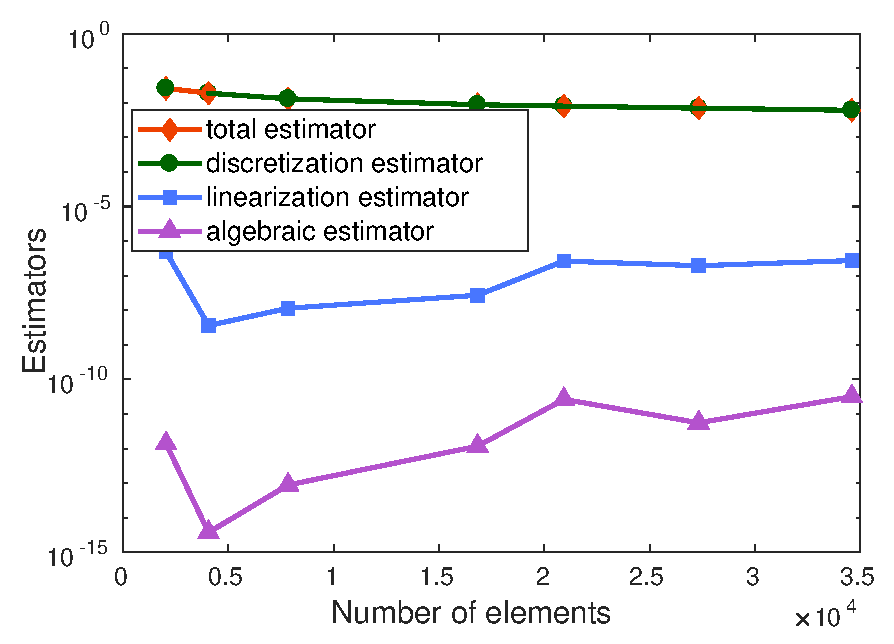
\includegraphics[width=\textwidth]{fig_article_chap_1/exact_resolution_convergence_estimator_number_elements.eps}    
%\label{ref:position_membrane_convergence}
\end{minipage}\hfill
\begin{minipage}[c]{.333\linewidth}
   \centering
   \quad \small{Inexact Newton} \hspace{3 cm} \scriptsize{(\textcolor{midnightblue}{$\left\|\bR_{\mathrm{rel,alg}}^{\kk,\ii}\right\| \leq \left\|\bR_{\mathrm{rel,lin}}^{\kk,\ii}\right\|$, $\left\|\bR_{\mathrm{rel,lin}}^{\kk,\ii}\right\| \leq 10^{-10}$})}
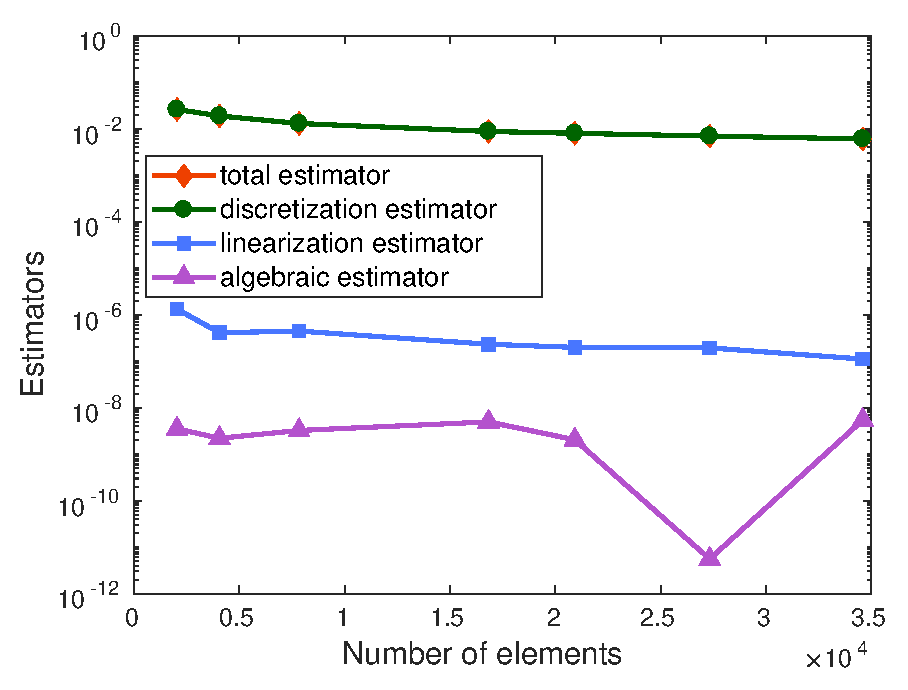
\includegraphics[width=\textwidth]{fig_article_chap_1/inexact_resolution_convergence_estimator_number_elements.eps}    
%\label{ref:position_membrane_convergence}
\end{minipage}\hfill
\begin{minipage}[c]{.33\linewidth}
   \centering
   \small{\small{Adaptive Inexact Newton} \hspace{3 cm} \scriptsize{\textcolor{midnightblue}{($\gammalin=10^{-1}$, $\gammaalg=10^{-1}$)}}}
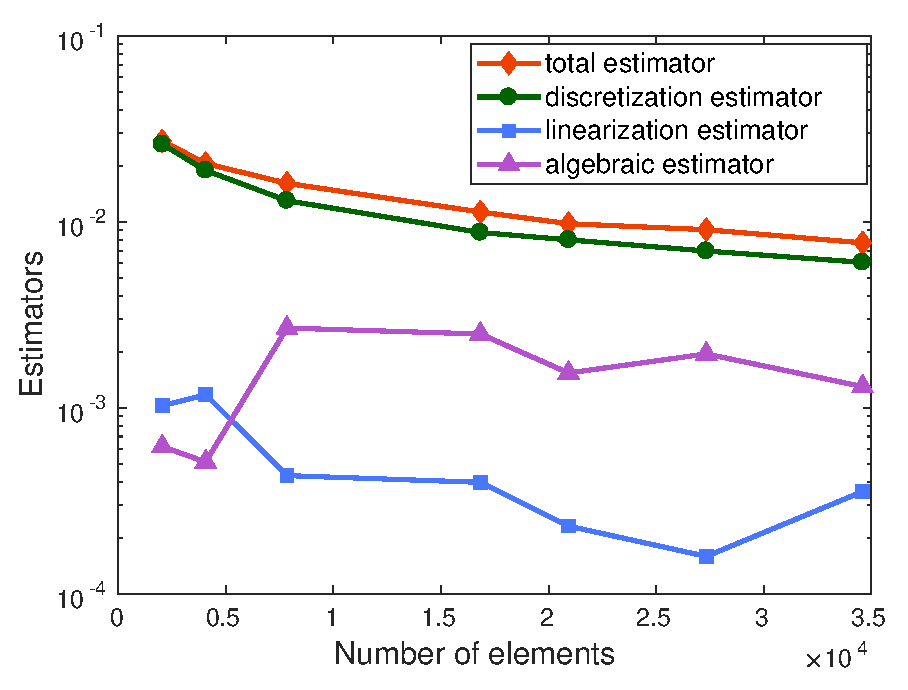
\includegraphics[width=\textwidth]{fig_article_chap_1/adapt_inexact_resolution_convergence_estimator_number_elements.eps}     
%\label{ref:lambda_membrane_convergence} 
\end{minipage}
%\caption{Exact Newton(left), Inexact Newton(middle), adaptive inexact Newton(right)}
\end{figure}

\textcolor{red}{\textbf{Precision is preserved for adaptive inexact semismooth Newton method.}}


\end{frame}

\begin{frame}
\frametitle{Adaptivity}
\hspace{5.5 cm} Exact Newton/Adaptive inexact Newton \hspace{3.5 cm } 
%Inexact Newton
\begin{figure}
   \centering
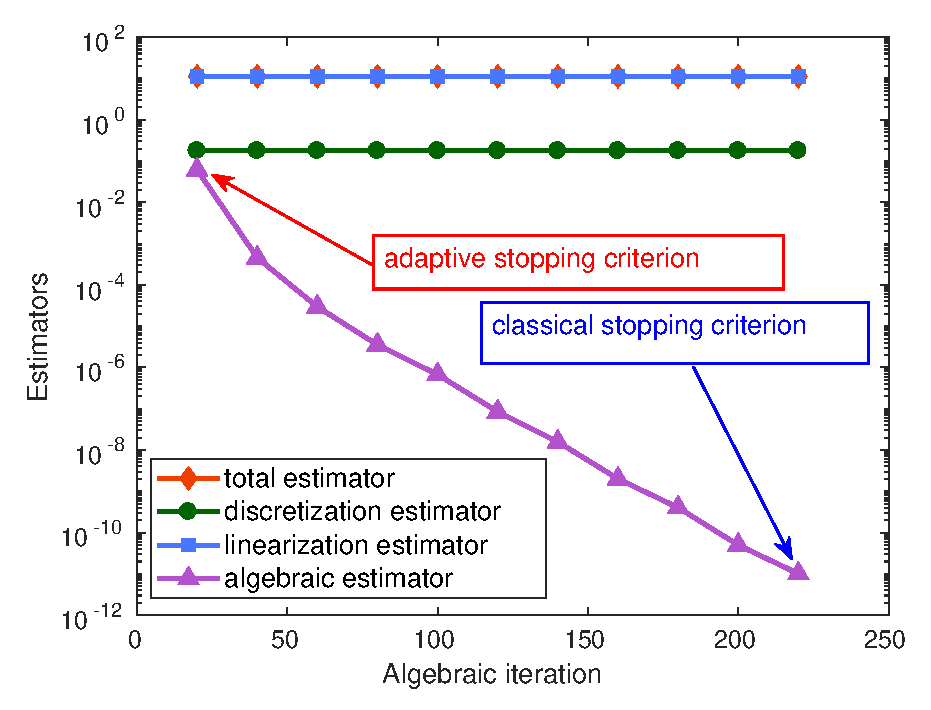
\includegraphics[width=0.50\textwidth]{fig_article_chap_1/exact_adapt_res_estimators_gmres_iter_first_newton_iter_Hmax_015.eps}    
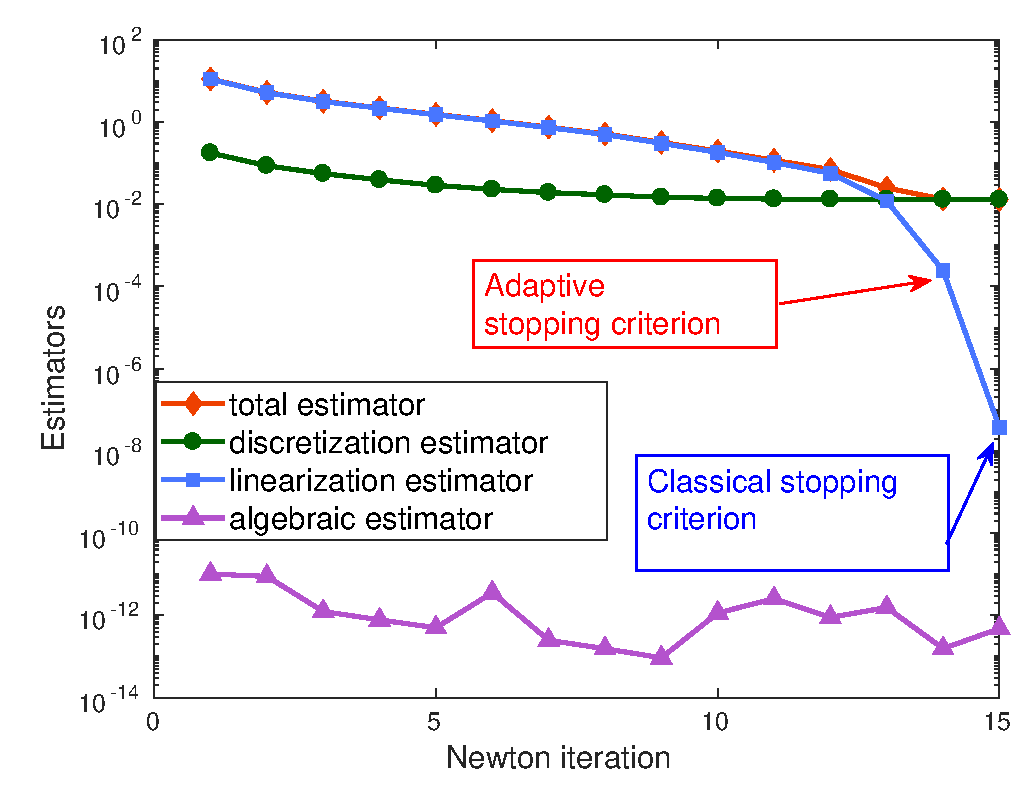
\includegraphics[width=0.49\textwidth]{fig_article_chap_1/exact_adapt_resolution_estimators_newton_iter_Hmax_015.eps} 
\end{figure}
\end{frame}
%% ESTIMATORS INEX NEWTON
% \begin{frame}
% \frametitle{Newton-min adaptivity}
% \hspace{2 cm} Exact/Adapt inexact Newton \hspace{3.5 cm } Inexact Newton\begin{figure}
% 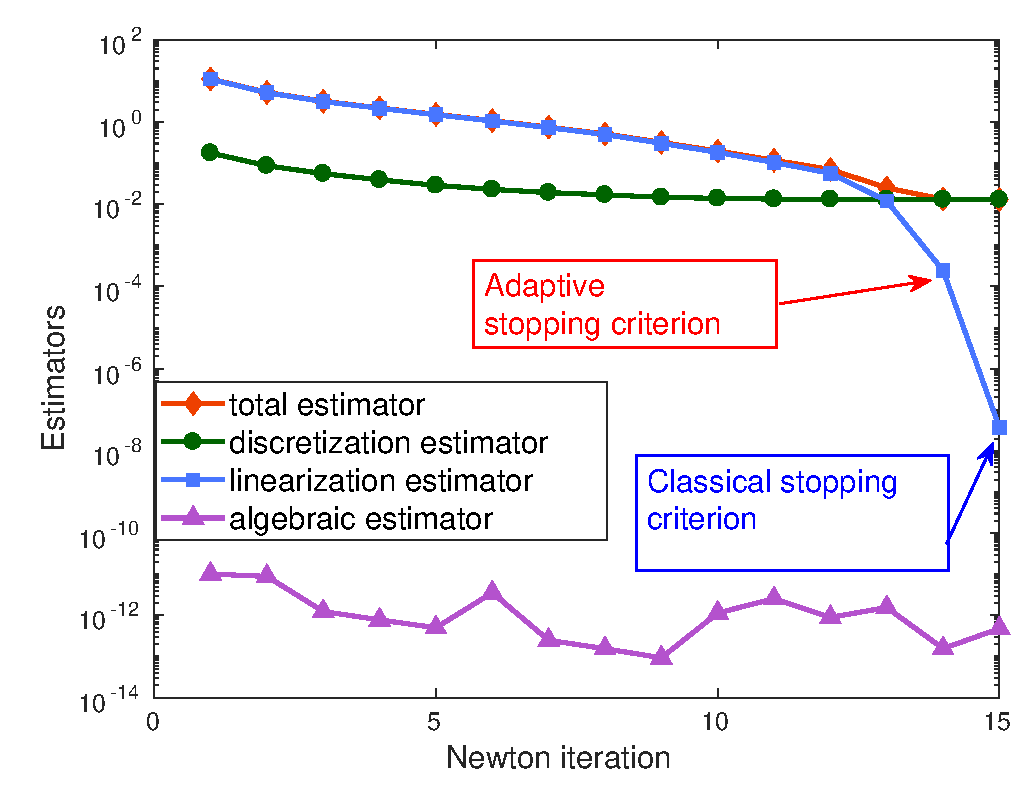
\includegraphics[width=0.5\textwidth]{fig_article_chap_1/exact_adapt_resolution_estimators_newton_iter_Hmax_015.eps}    
% 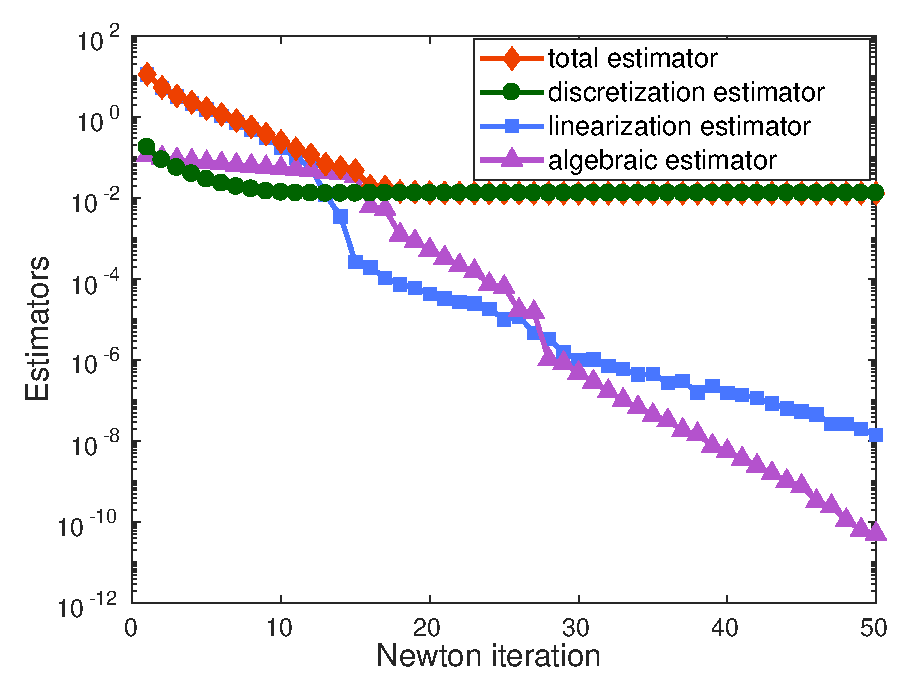
\includegraphics[width=0.5\textwidth]{fig_article_chap_1/inexacte_resolution_Hmax_015_estimators_newton_step.eps}     
% \end{figure}
% \end{frame}

\begin{frame}
\frametitle{Overall performance}
\begin{figure}
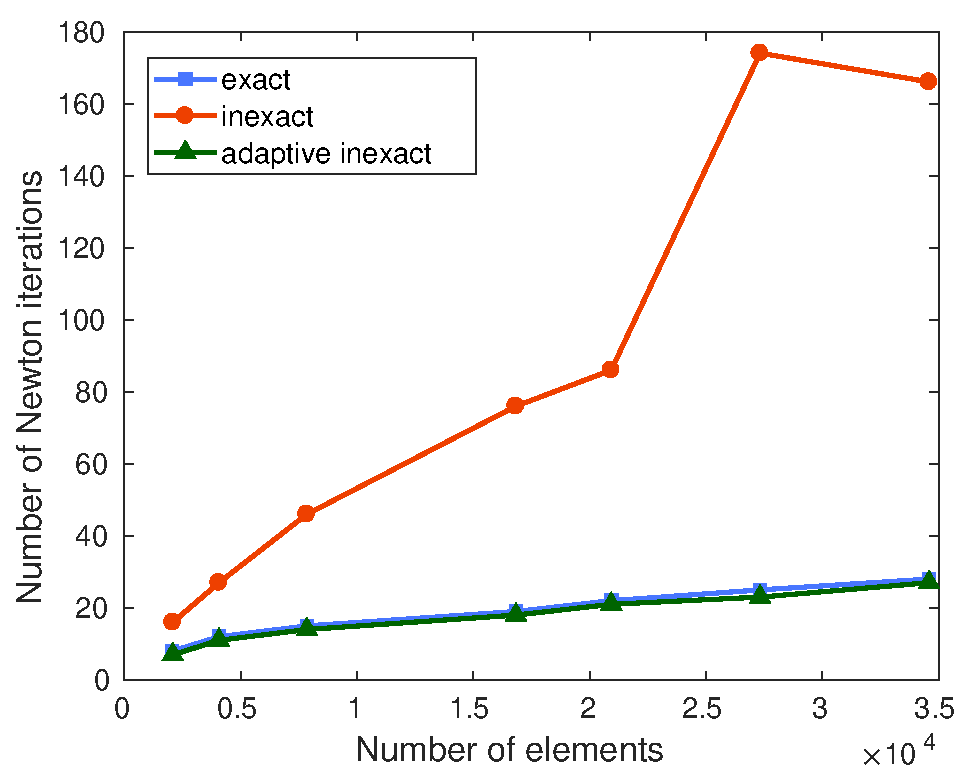
\includegraphics[width=0.47\textwidth]{fig_article_chap_1/comparison_three_methods_number_Newton_iter_number_elements.eps}  \quad  
 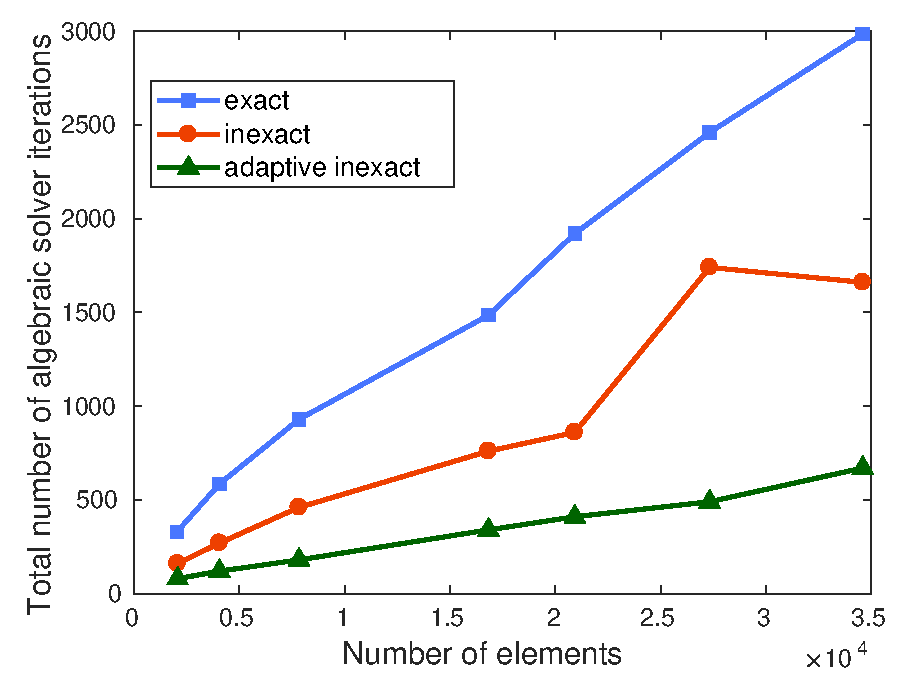
\includegraphics[width=0.50\textwidth]{fig_article_chap_1/comparison_three_methods_total_number_Newton_Gmres_iter_number_elements.eps}     
\end{figure}
\end{frame}


\begin{frame}
  \hspace{0.5 cm}\textcolor{red}{\textbf{Effectivity indices:}} $\mathrm{I}_{\mathrm{eff}} \egaldef \frac{\eta^{\kk,\ii}}{\tnorm{\bu-\bu_h^{\kk,\ii}}_{\Omega}}$ \hspace{3 cm} \textcolor{red}{\textbf{contact estimator}}
\begin{figure}
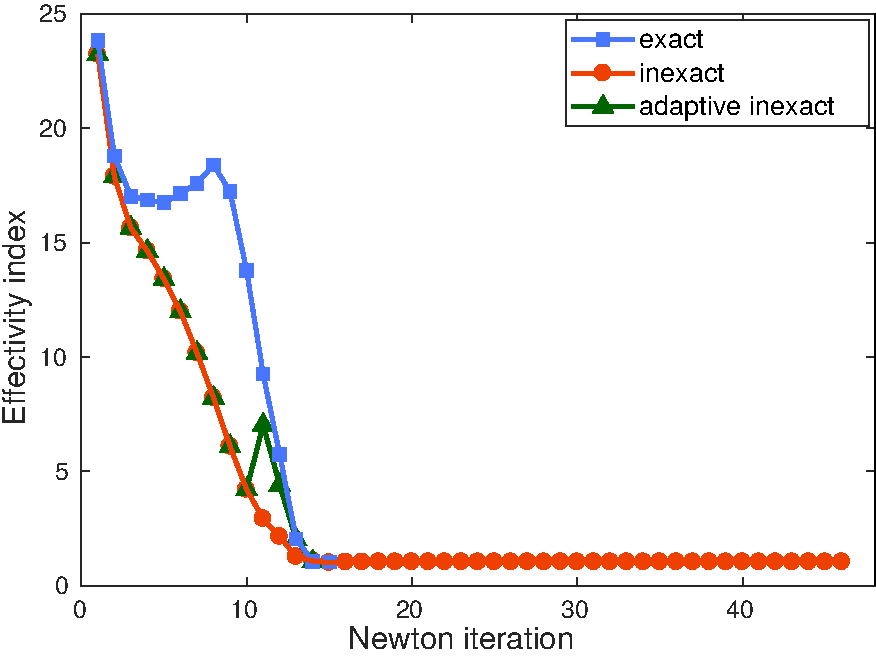
\includegraphics[width=0.47 \textwidth]{fig_article_chap_1/effectivity_index_3_methods_Hmax_015.pdf}   \quad 
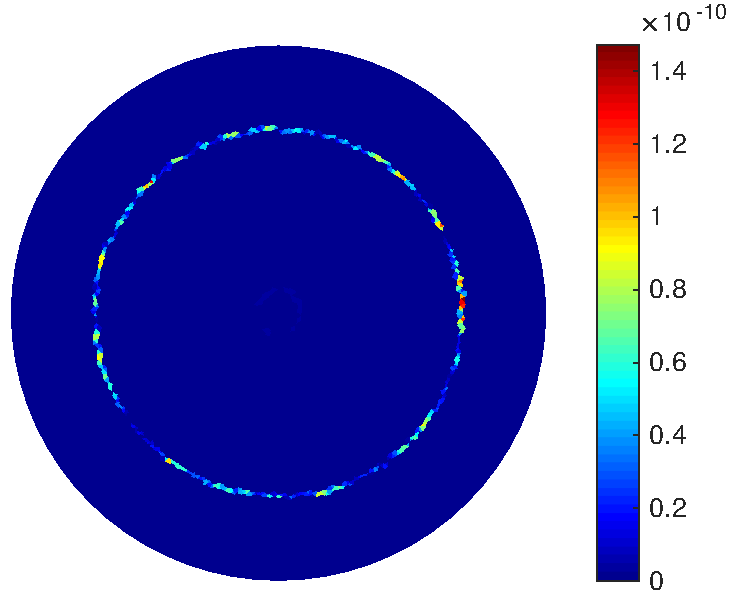
\includegraphics[width=0.50\textwidth]{fig_article_chap_1/modif_fig_contact_estimator_hmax0,09_Dt0,001_tt180}     
\end{figure}
\end{frame}

% \begin{frame}
%  \hspace{1 cm}\textcolor{red}{\textbf{Local distribution of the error}} \hspace{2.5 cm}    \textcolor{red}{\textbf{Local error estimator}}
% \begin{figure}
% 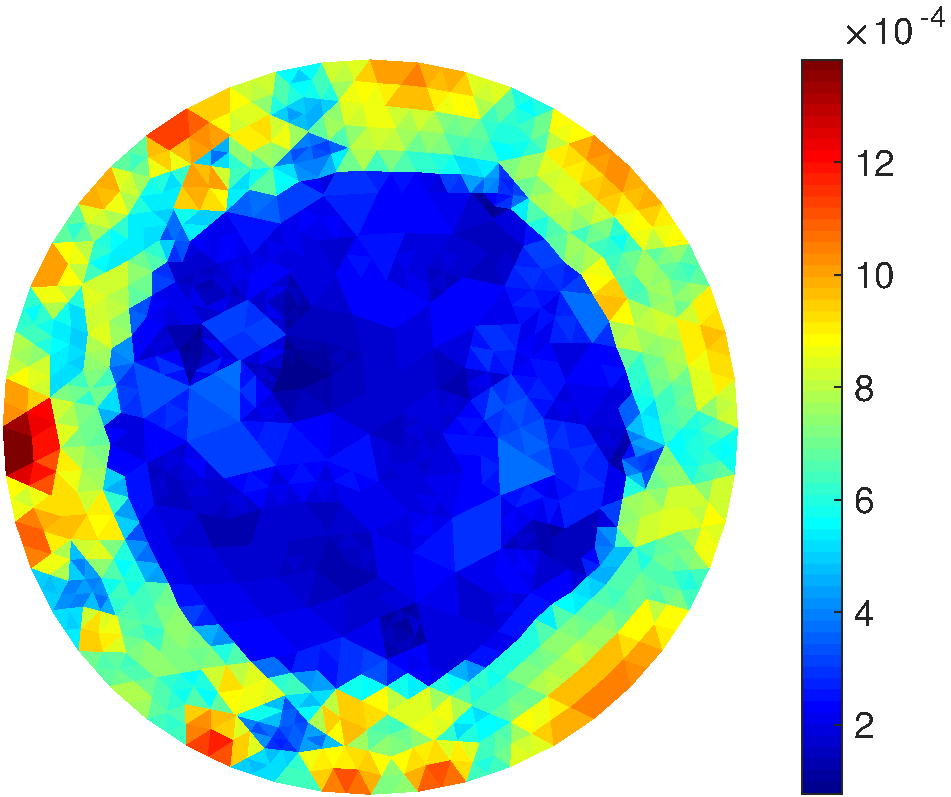
\includegraphics[width=0.47 \textwidth]{fig_article_chap_1/energy_norm_second_level_inexact_newton_iter_30.pdf}  
% 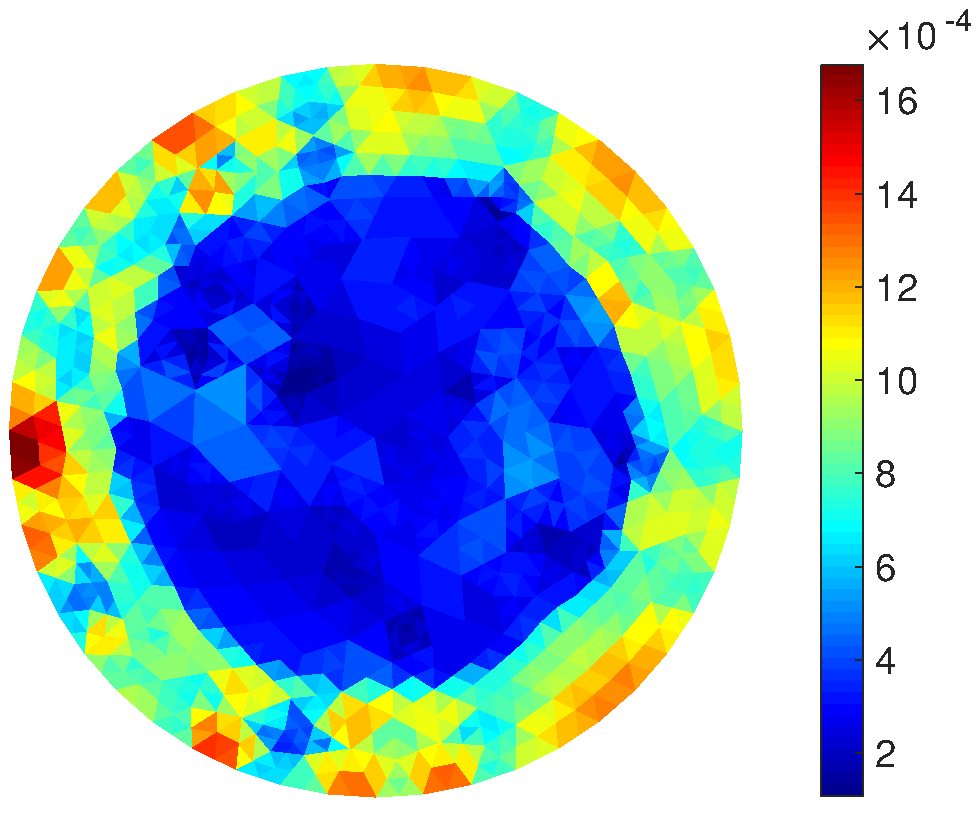
\includegraphics[width=0.48 \textwidth]{fig_article_chap_1/estimator_actual_error_inexact_newton_iter_30second_level.pdf} 
% \end{figure}
% \end{frame}
%
